\documentclass[a4paper,12pt]{article}

\usepackage{graphicx}
\usepackage{amsmath}
\usepackage{hyperref}
\usepackage{caption}
\usepackage{subcaption}
\usepackage{circuitikz}
\usepackage{longtable} 
\usepackage{tikz}

\title{\textbf{Lab Report: Experiment 4}}
\author{EE24BTECH11003 : Akshara Sarma Chennubhatla\\EE24BTECH11005 : Arjun Pavanje}

\begin{document}
\maketitle
\begin{center}
	\textbf{Experiment:}\\Studying damped\\LC oscillations\\for underdamped conditions
\end{center}
\vspace{30pt}
\begin{figure}[h!]
	\centering
	
\includegraphics[width = 100pt]{.logo/logo.png}\\
\end{figure}
\begin{center}
	Bachelor of Technology\\
	\vspace{10pt}
	Department of Electrical Engineering\\
\end{center}
\newpage

\section{Introduction}
In this experiment, we study and analyze the transient response of an LC circuit, determine the natural frequency ($\omega_n$), and calculate the damping ratio ($\xi$) using theoretical and experimental methods. \newline An LC circuit consists of an inductor (L) and a capacitor (C) connected in parallel. When a charged capacitor is connected to an inductor, energy oscillates between the capacitor's electric field and the inductor's magnetic field. The system follows the second-order differential equation.

\begin{itemize}
    \item Inductance, $2.2 mH$ 
    \item Capacitance, $ 4.6 nF $
\end{itemize}

\section{Theory}
\begin{figure}[!h]
\centering
\resizebox{0.5\textwidth}{!}{%
\begin{circuitikz}
\tikzstyle{every node}=[font=\small]
\draw (6.25,14.75) to[C,l={ \small $460pF$}] (6.25,11);
\draw (10,14.75) to[L,l={ \small $2.2mH, 55\Omega$} ] (10,11);
\draw (6.25,14.75) to[short] (10,14.75);
\draw (6.25,11) to[short] (10,11);
\end{circuitikz}
}%
\label{fig:my_label}
\end{figure}
Writing $KVL$ equation, 
\begin{align*}
    L \frac{di}{dt} + iR + \frac{1}{C} \int i \, dt &= 0 \\[10pt]
    L \frac{d^2q}{dt^2} + R \frac{dq}{dt} + \frac{q}{C} &= 0 \\[10pt]
    \frac{d^2q}{dt^2} + \left(\frac{R}{L}\right) \frac{dq}{dt} + \frac{q}{LC} &= 0
\end{align*}

Let 
\begin{align*}
    \omega_n &= \frac{1}{\sqrt{LC}}, \\ 
    \xi &= \frac{R}{2} \sqrt{\frac{C}{L}}.
\end{align*}

Substituting these into the equation:
\begin{align*}
    \frac{d^2q}{dt^2} + 2\xi \omega_n \frac{dq}{dt} + (\omega_n^2) q &= 0
\end{align*}

Here, $\xi < 1$, so the system is underdamped.

The solution for $q(t) = e^{st}$ will have complex conjugate roots:
\begin{align*}
    s &= -\xi \omega_n \pm j\omega_d,
\end{align*}
where $\omega_d = \omega_n \sqrt{1 - \xi^2}$.

Thus, the current $i(t)$ can be written as:
\begin{align*}
    q &= Ce^{-\xi \omega_n t} e^{j\omega_d t} + C^{*}e^{-\xi \omega_n t} e^{-j\omega_d t}
\end{align*}
Expanding this:
\begin{align*}
    q &=A e^{-\xi \omega_n t} \cos(\omega_d t + \phi) .
\end{align*}
$\phi, A$ are constants that can be determined using inital conditions. We know $i\Bigr|_{t=0} = 0$, and $q\Bigr|_{t=0} = CV_{DC}$\newline\newline
Substituting $q(0) = CV_{DC}$,
\begin{align*}
    CV_{DC} &= A \cos(\phi). \tag{1}
\end{align*}
The current $i(t)$ is given by,
\begin{align*}
    i(t) &= \frac{dq}{dt}, \\[5pt]
    i(t) &= -A e^{-\xi \omega_n t} (\xi \omega_n \cos(\omega_d t + \phi) + \omega_d \sin(\omega_d t + \phi)).
\end{align*}
At $t = 0$,
\begin{align*}
    i(0) &= -A (\xi \omega_n \cos(\phi) + \omega_d \sin(\phi)).
\end{align*}
Substituting $\frac{dq}{dt}\Bigr|_{t=0} = 0$,
\begin{align*}
    0 &= -A (\xi \omega_n \cos(\phi) + \omega_d \sin(\phi)).
\end{align*}
Simplifying,
\begin{align*}
    0 &= \xi \omega_n \cos(\phi) + \omega_d \sin(\phi). \tag{2}
\end{align*}
From $(1), (2)$ we get,
\begin{align*}
   \phi &= \tan^{-1}\left(-\frac{\xi \omega_n}{\omega_d}\right)\\
   A &= \frac{CV_{DC}}{\cos(\phi)}
\end{align*}
We finally get,
\begin{align*}
   V(t) &= \left(\frac{CV_{DC}}{\sqrt{1-\xi^2}} \right) e^{-\xi \omega_n t}\cos\left(\omega_d t + \tan^{-1}\left(-\frac{\xi \omega_n}{w_d}\right)\right). 
\end{align*}
Where, $\xi = \frac{R}{2}\sqrt{\frac{C}{L}}, \omega_n = \frac{1}{\sqrt{LC}}, \omega_d = \omega_n\sqrt{1-\xi^2}$
\section{Procedure}
\begin{itemize}
    \item First, fully charge the capacitor using a DC voltage source (here, we have used $5V$).
    \item Then carefully disconnect the capacitor from charging and connect it in parallel with an inductor (preferably one of large inductance). 
    \item Measure the voltage across either the inductor or capacitor (we have measured across inductor for convenience) using an oscilloscope. 
    \item Using the oscilloscope, set it in the $single$ mode and adjust the trigger level accordingly so that the voltage decay across the inductor (or capacitor) can be observed and captured properly. 
    \item Be careful not to charge the capacitor when it is connected in parallel to the inductor, as the inductor WILL melt.
\end{itemize}


\section{Experimental Data}
Resistance $55\Omega$,\newline
Capacitance $4.6nF$\newline
Inductance, $2.2mH$
\begin{figure}[h!]
	\begin{subfigure}[b]{100pt}
		\caption{Experimental plot}
		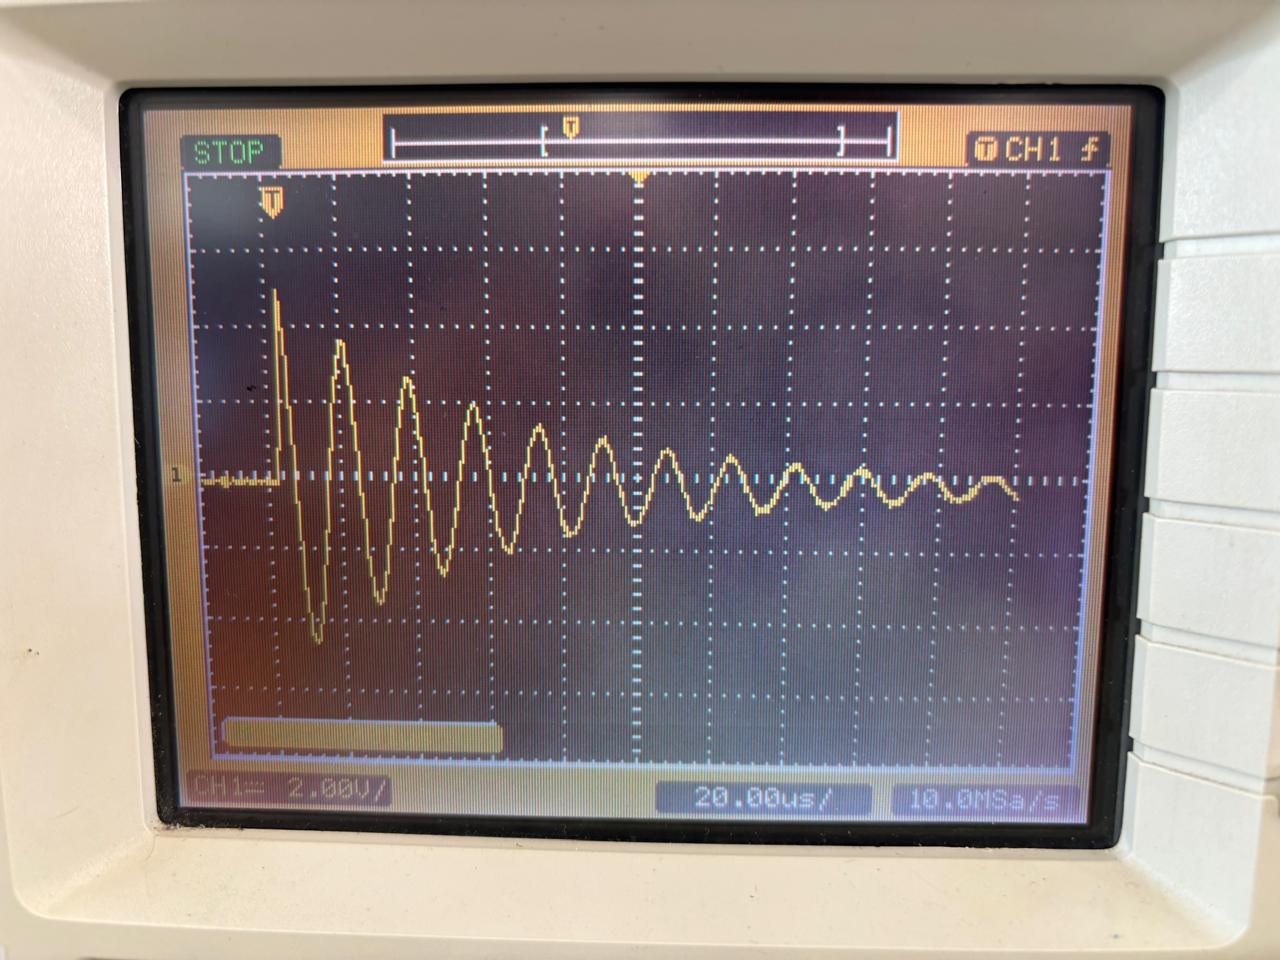
\includegraphics[width = 225pt]{figs/fig1.png}
	\end{subfigure}
	\hspace{110pt}
	\begin{subfigure}[b]{100pt}
		\caption{Theoretical plot}
		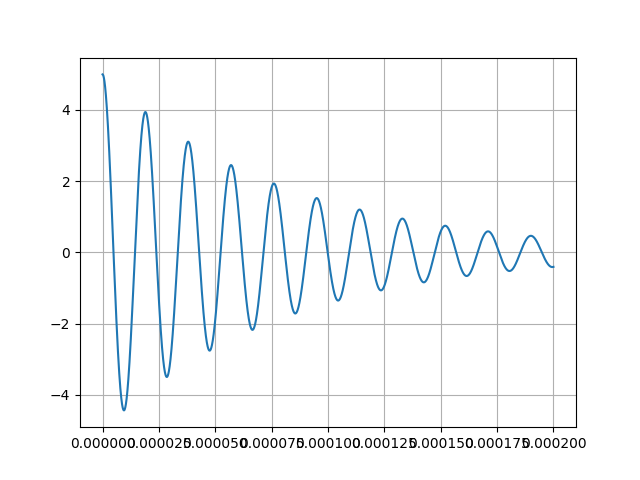
\includegraphics[width = 250pt]{figs/fig2.png}
	\end{subfigure}
\end{figure}
Below are the readings taken at different points in the plot to calculate the value of $\xi$ which we will then use to calculate the value of resistance. Then we will verify the obtained value with the labelled value of resistance on the inductor.
\pagebreak
\section{Measurements}
\begin{figure}[h!]
	\begin{subfigure}[b]{100pt}
		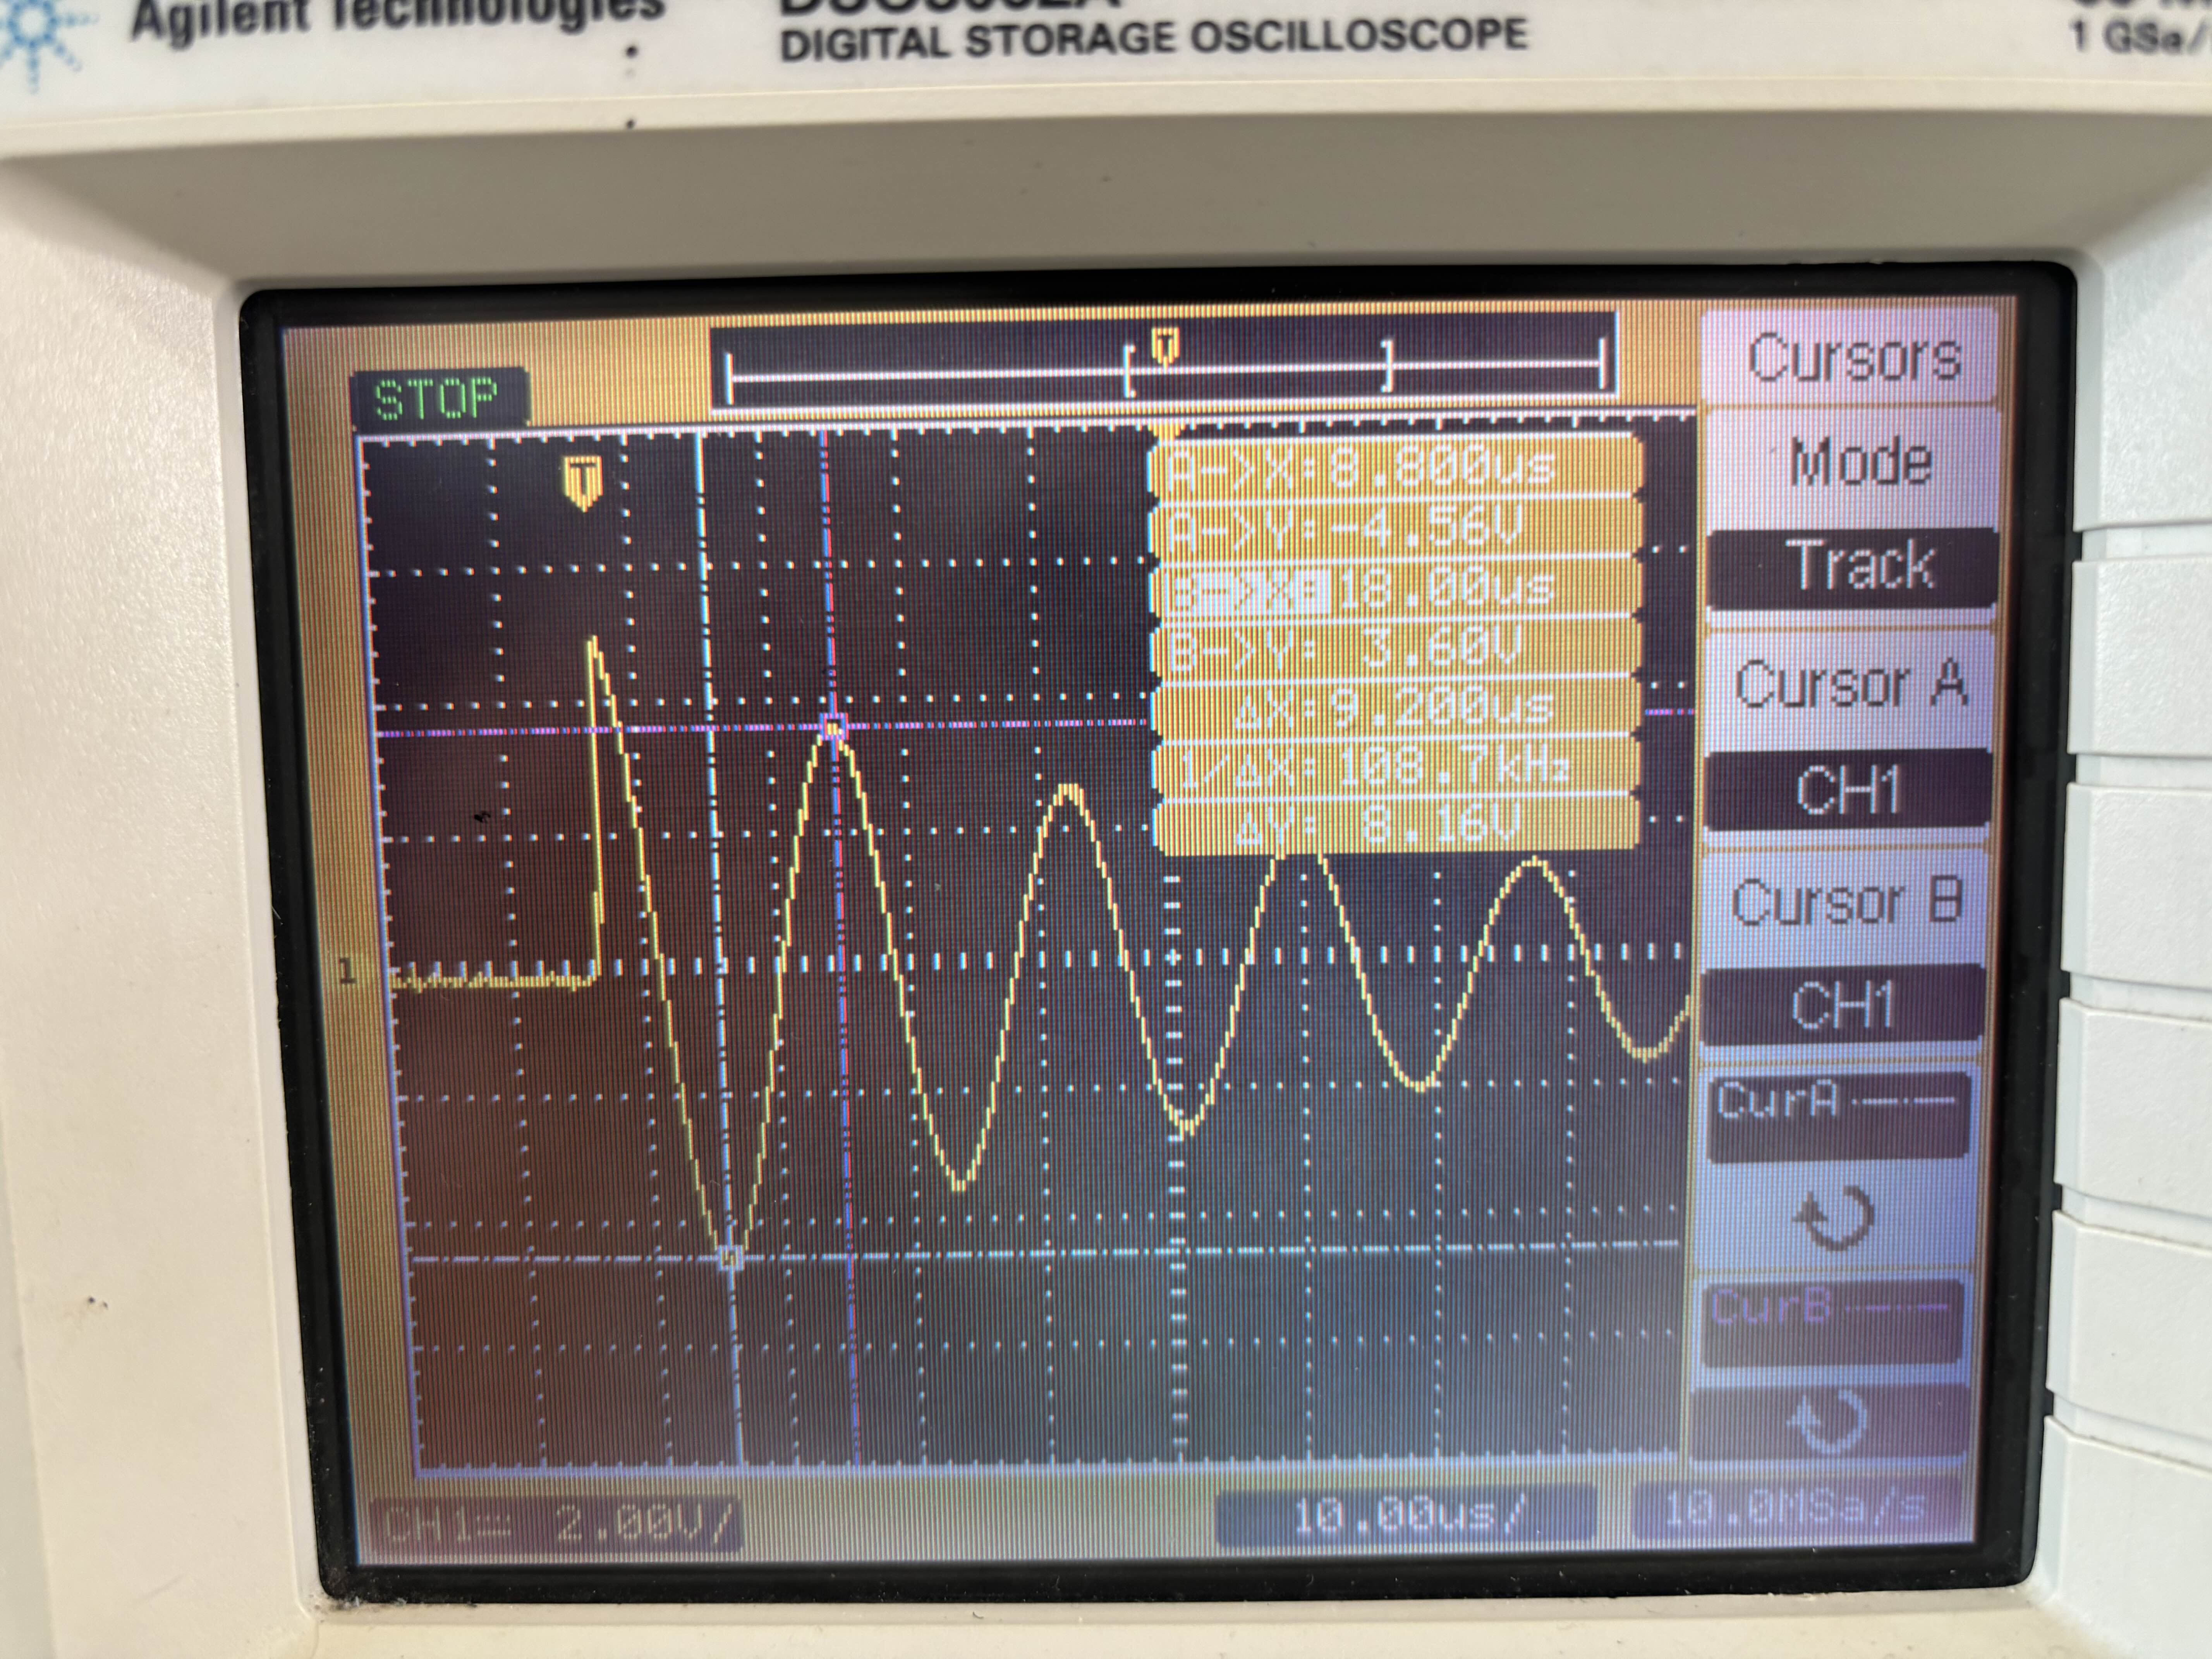
\includegraphics[width = 225pt]{figs/fig3.jpg}
	\end{subfigure}
	\hspace{110pt}
\begin{subfigure}[b]{100pt}
		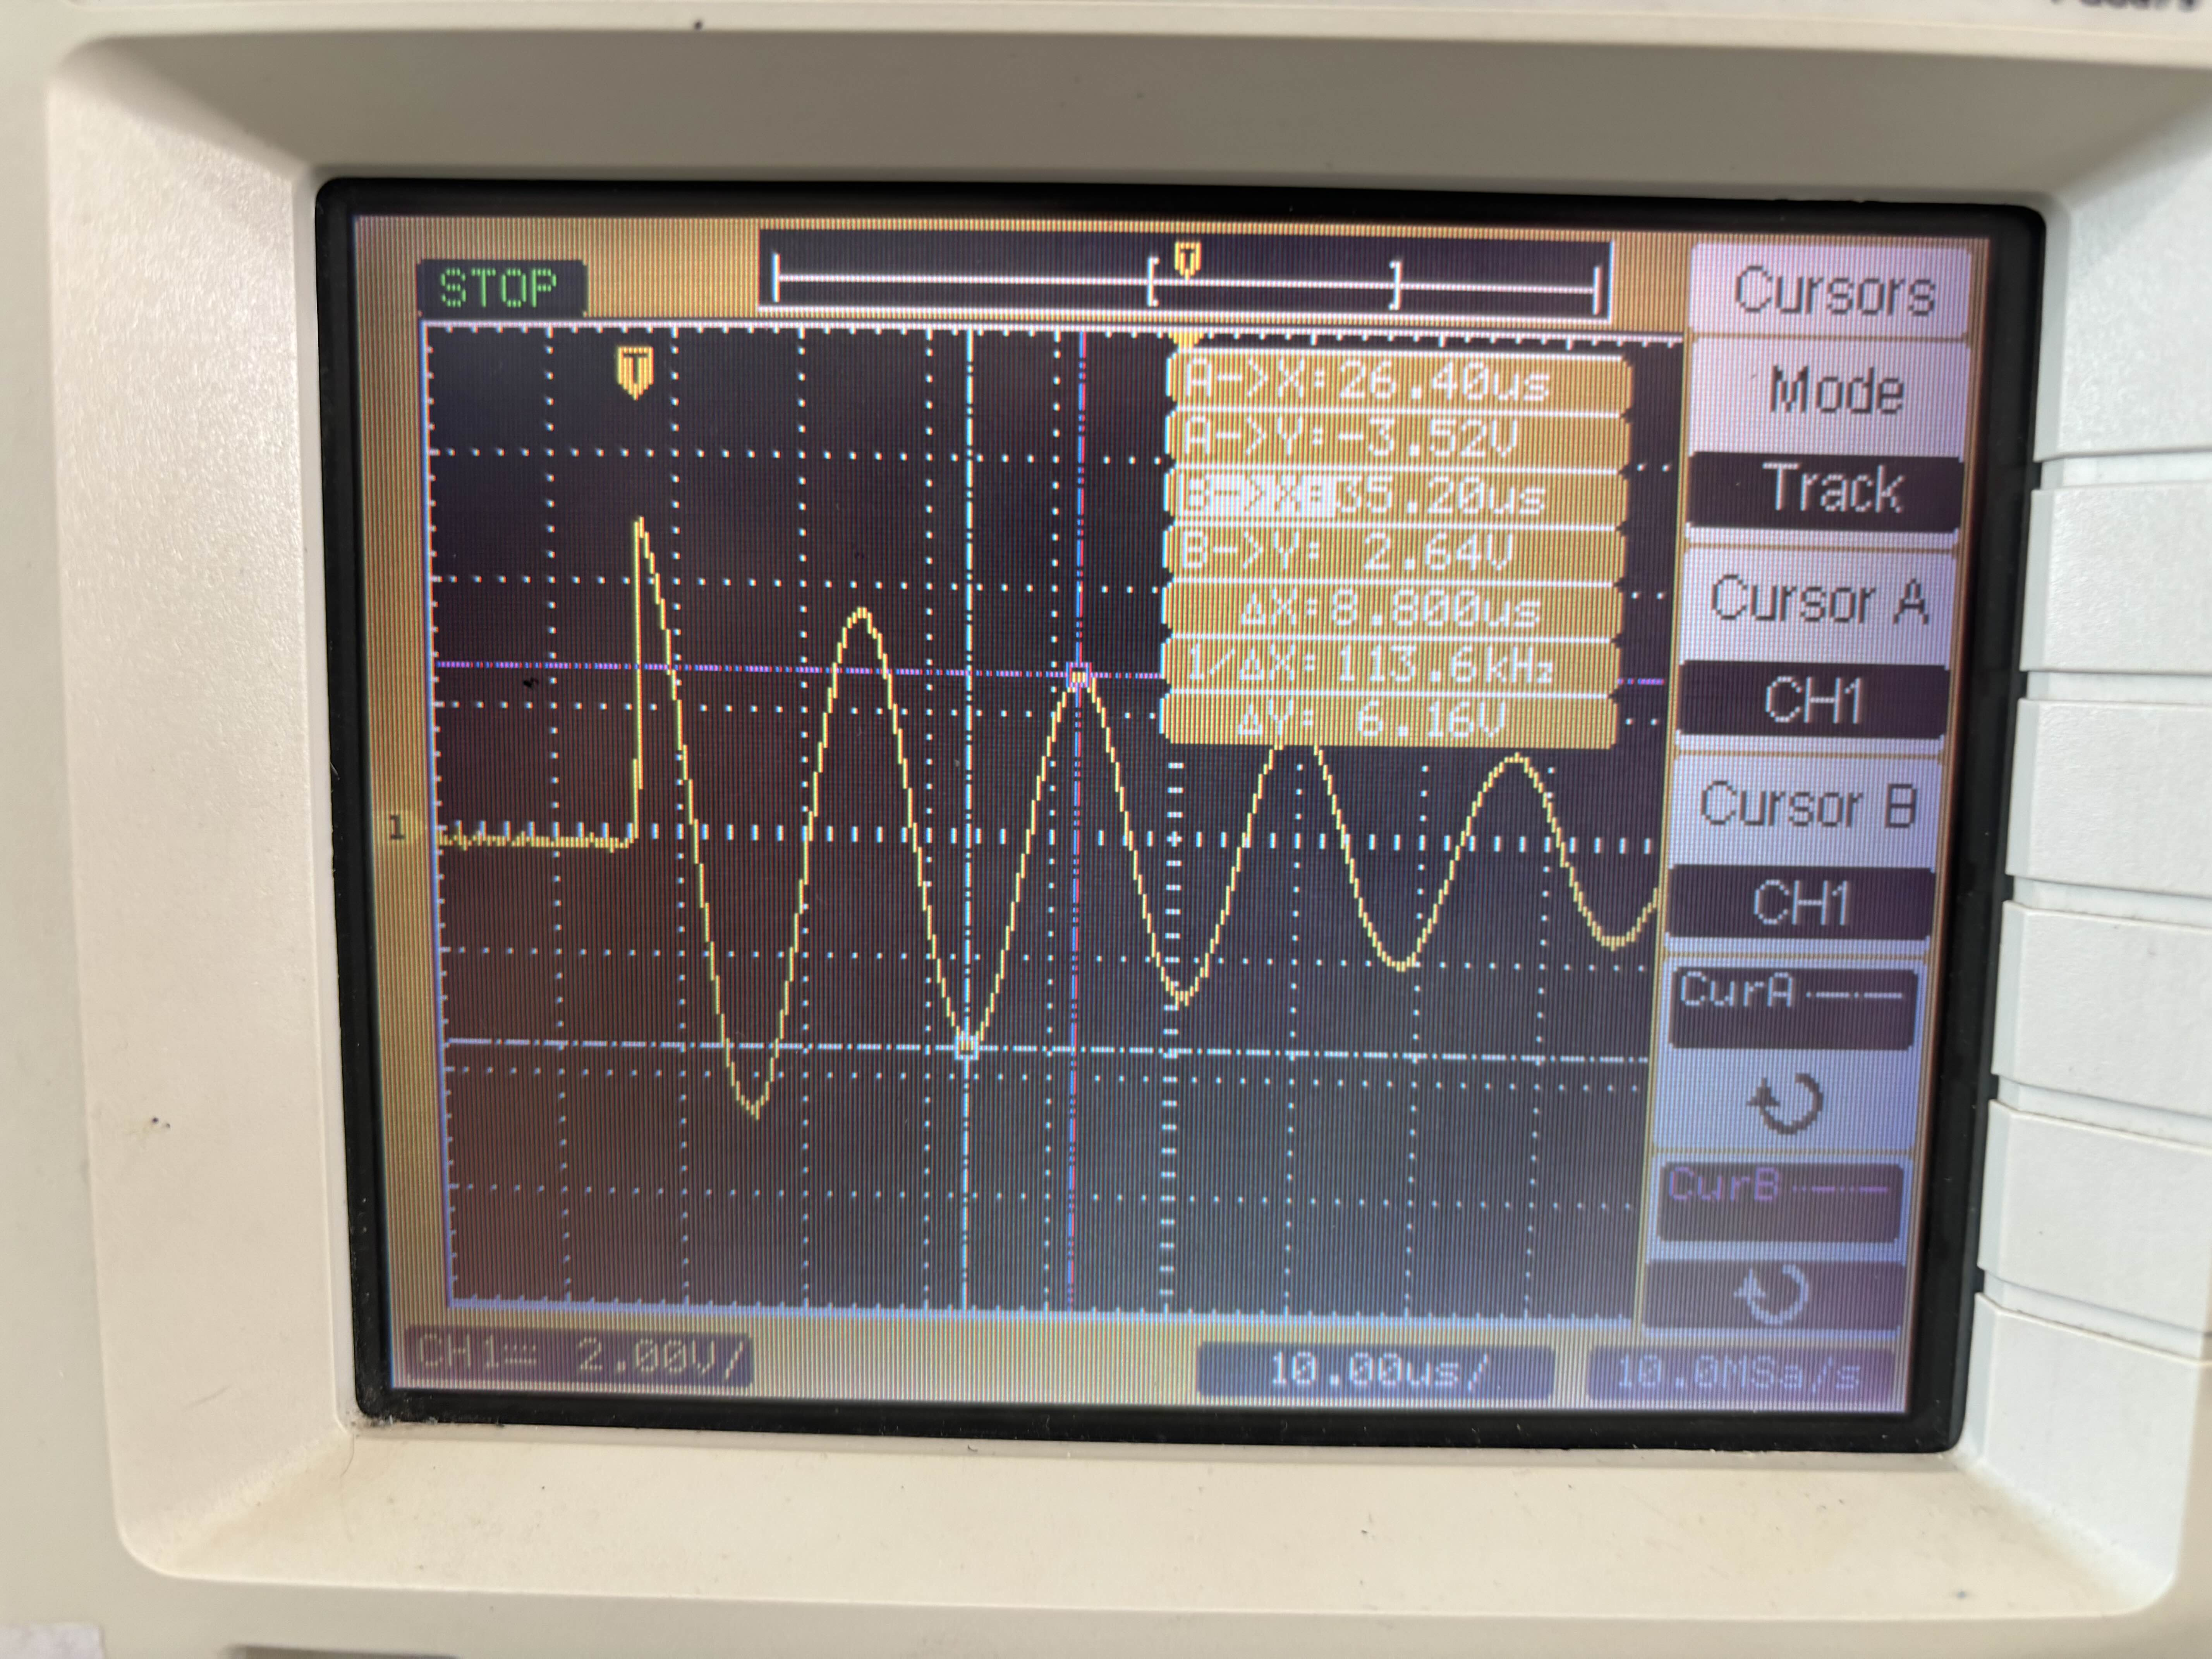
\includegraphics[width = 225pt]{figs/fig4.jpg}
	\end{subfigure}
\end{figure}
\pagebreak
\begin{figure}[h!]
\begin{subfigure}[b]{100pt}
		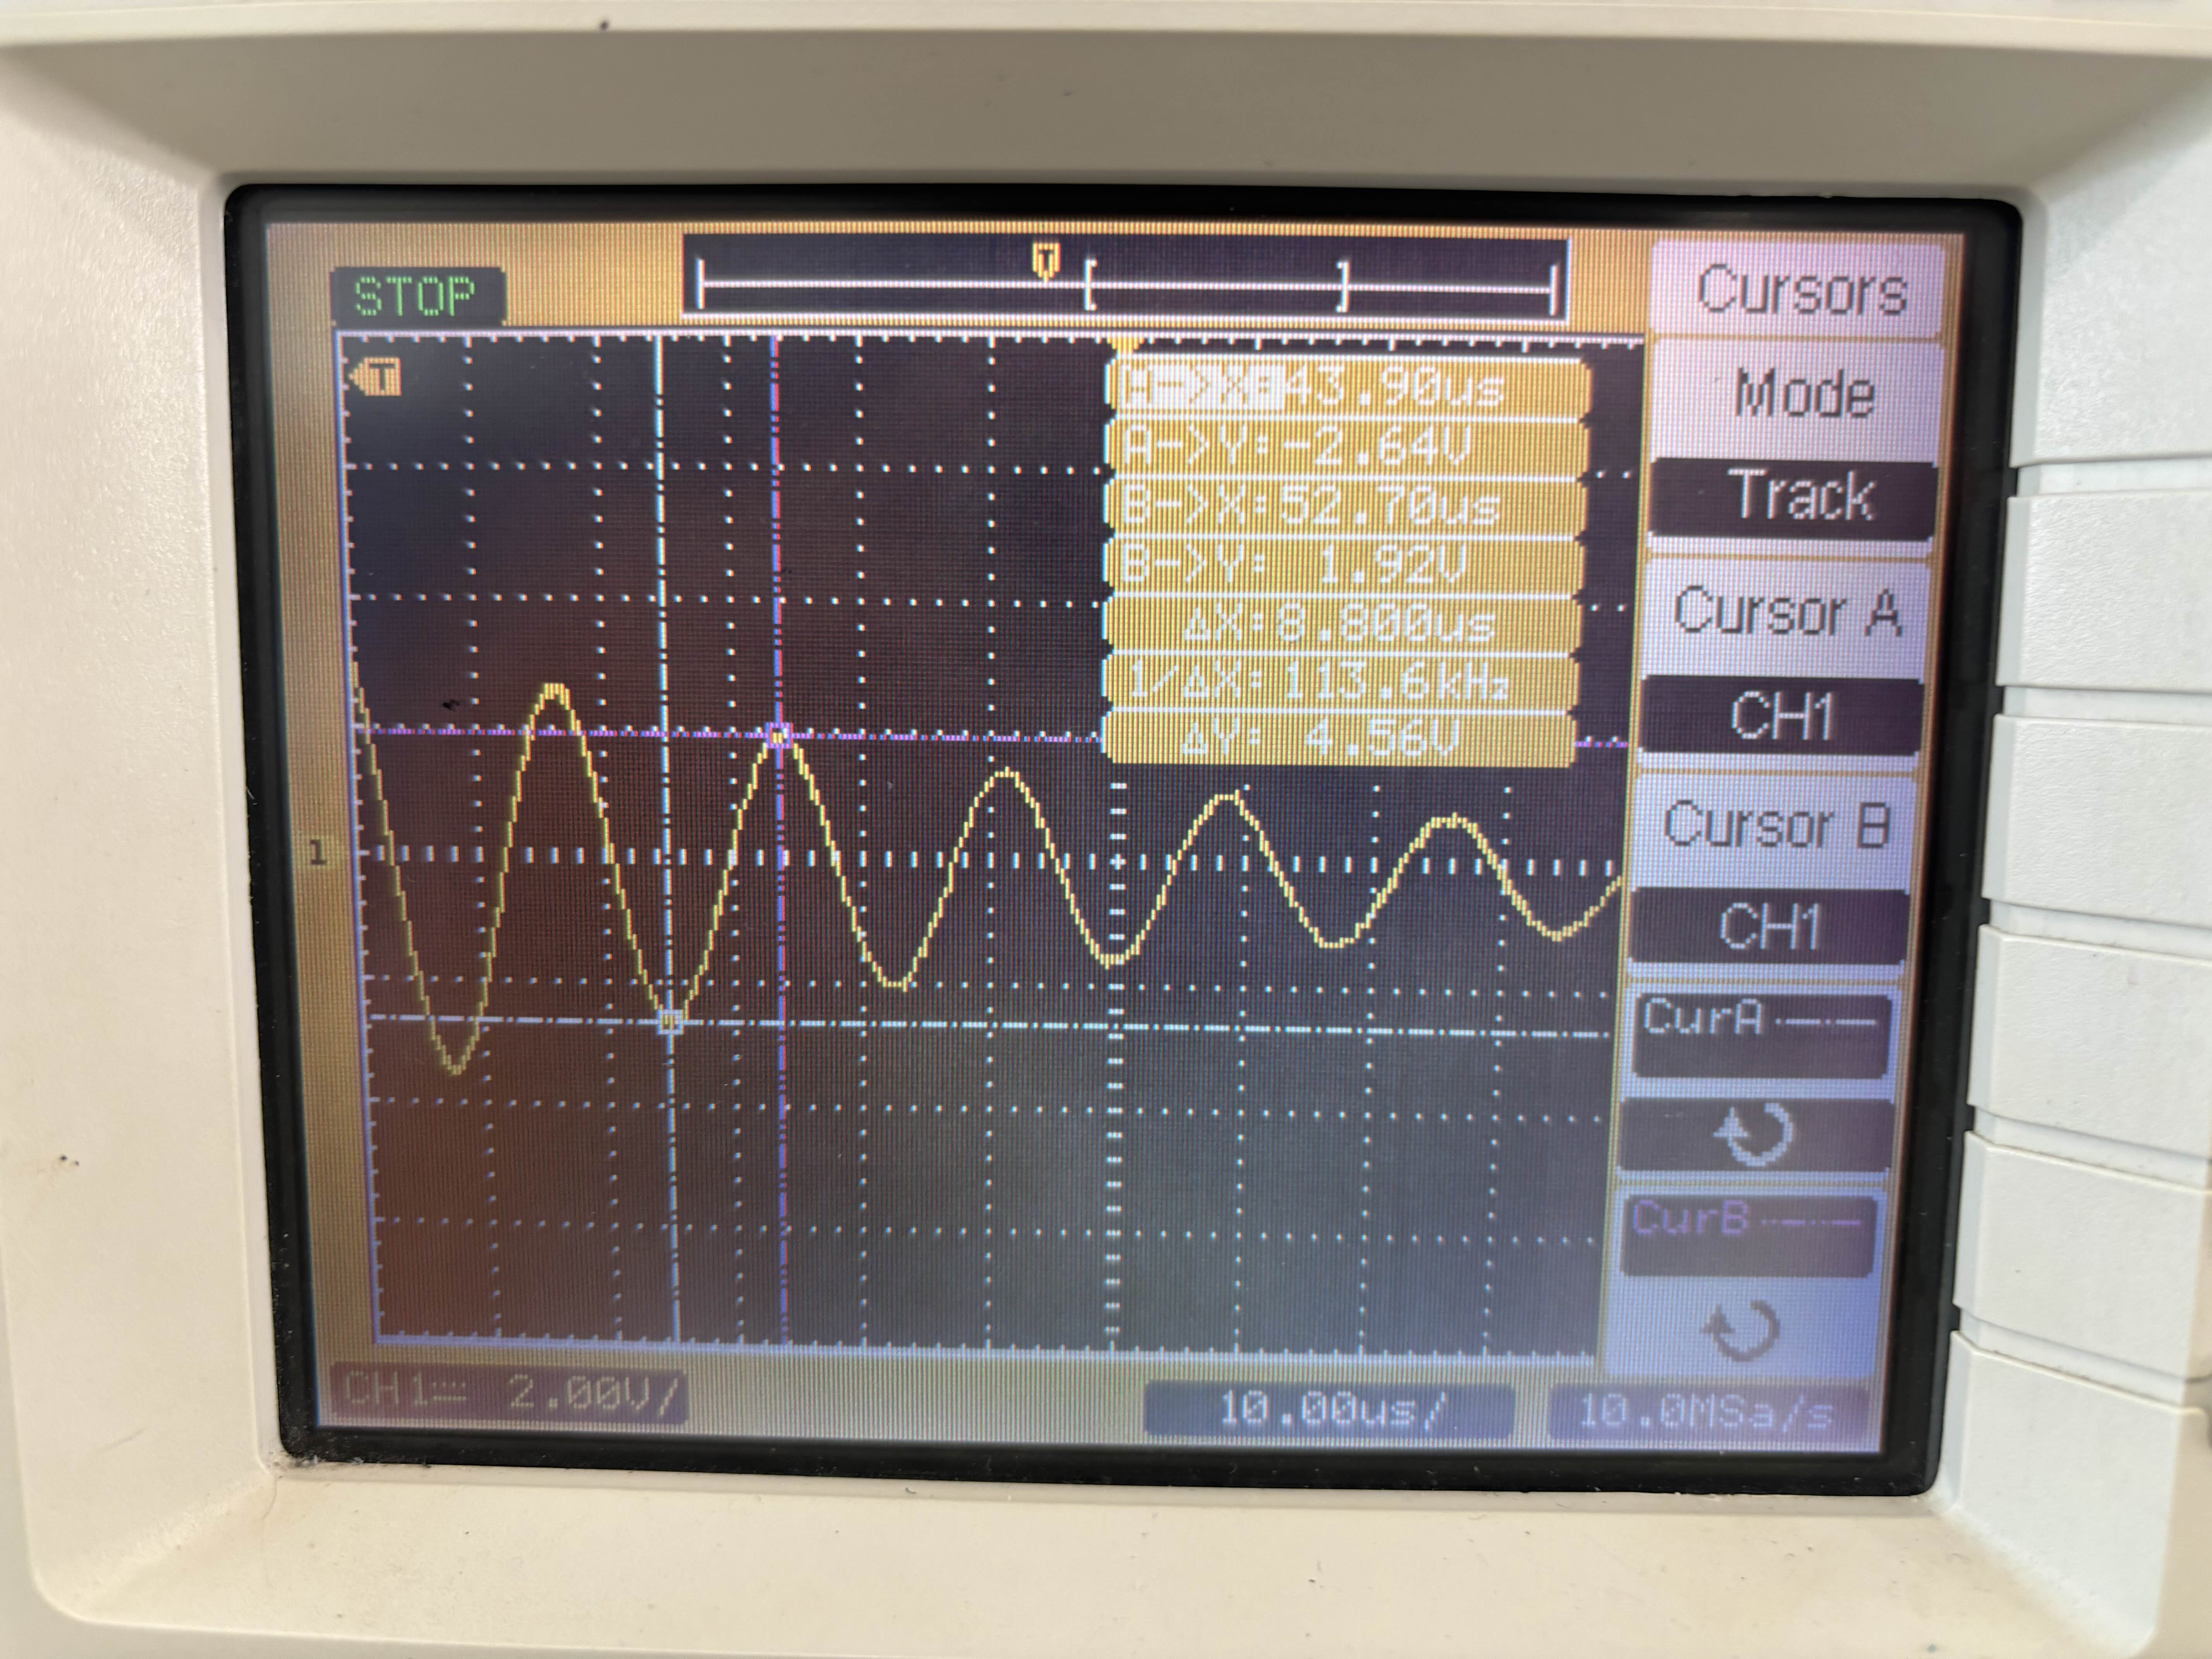
\includegraphics[width = 225pt]{figs/fig5.jpg}
	\end{subfigure}
	\hspace{110pt}
\begin{subfigure}[b]{100pt}
		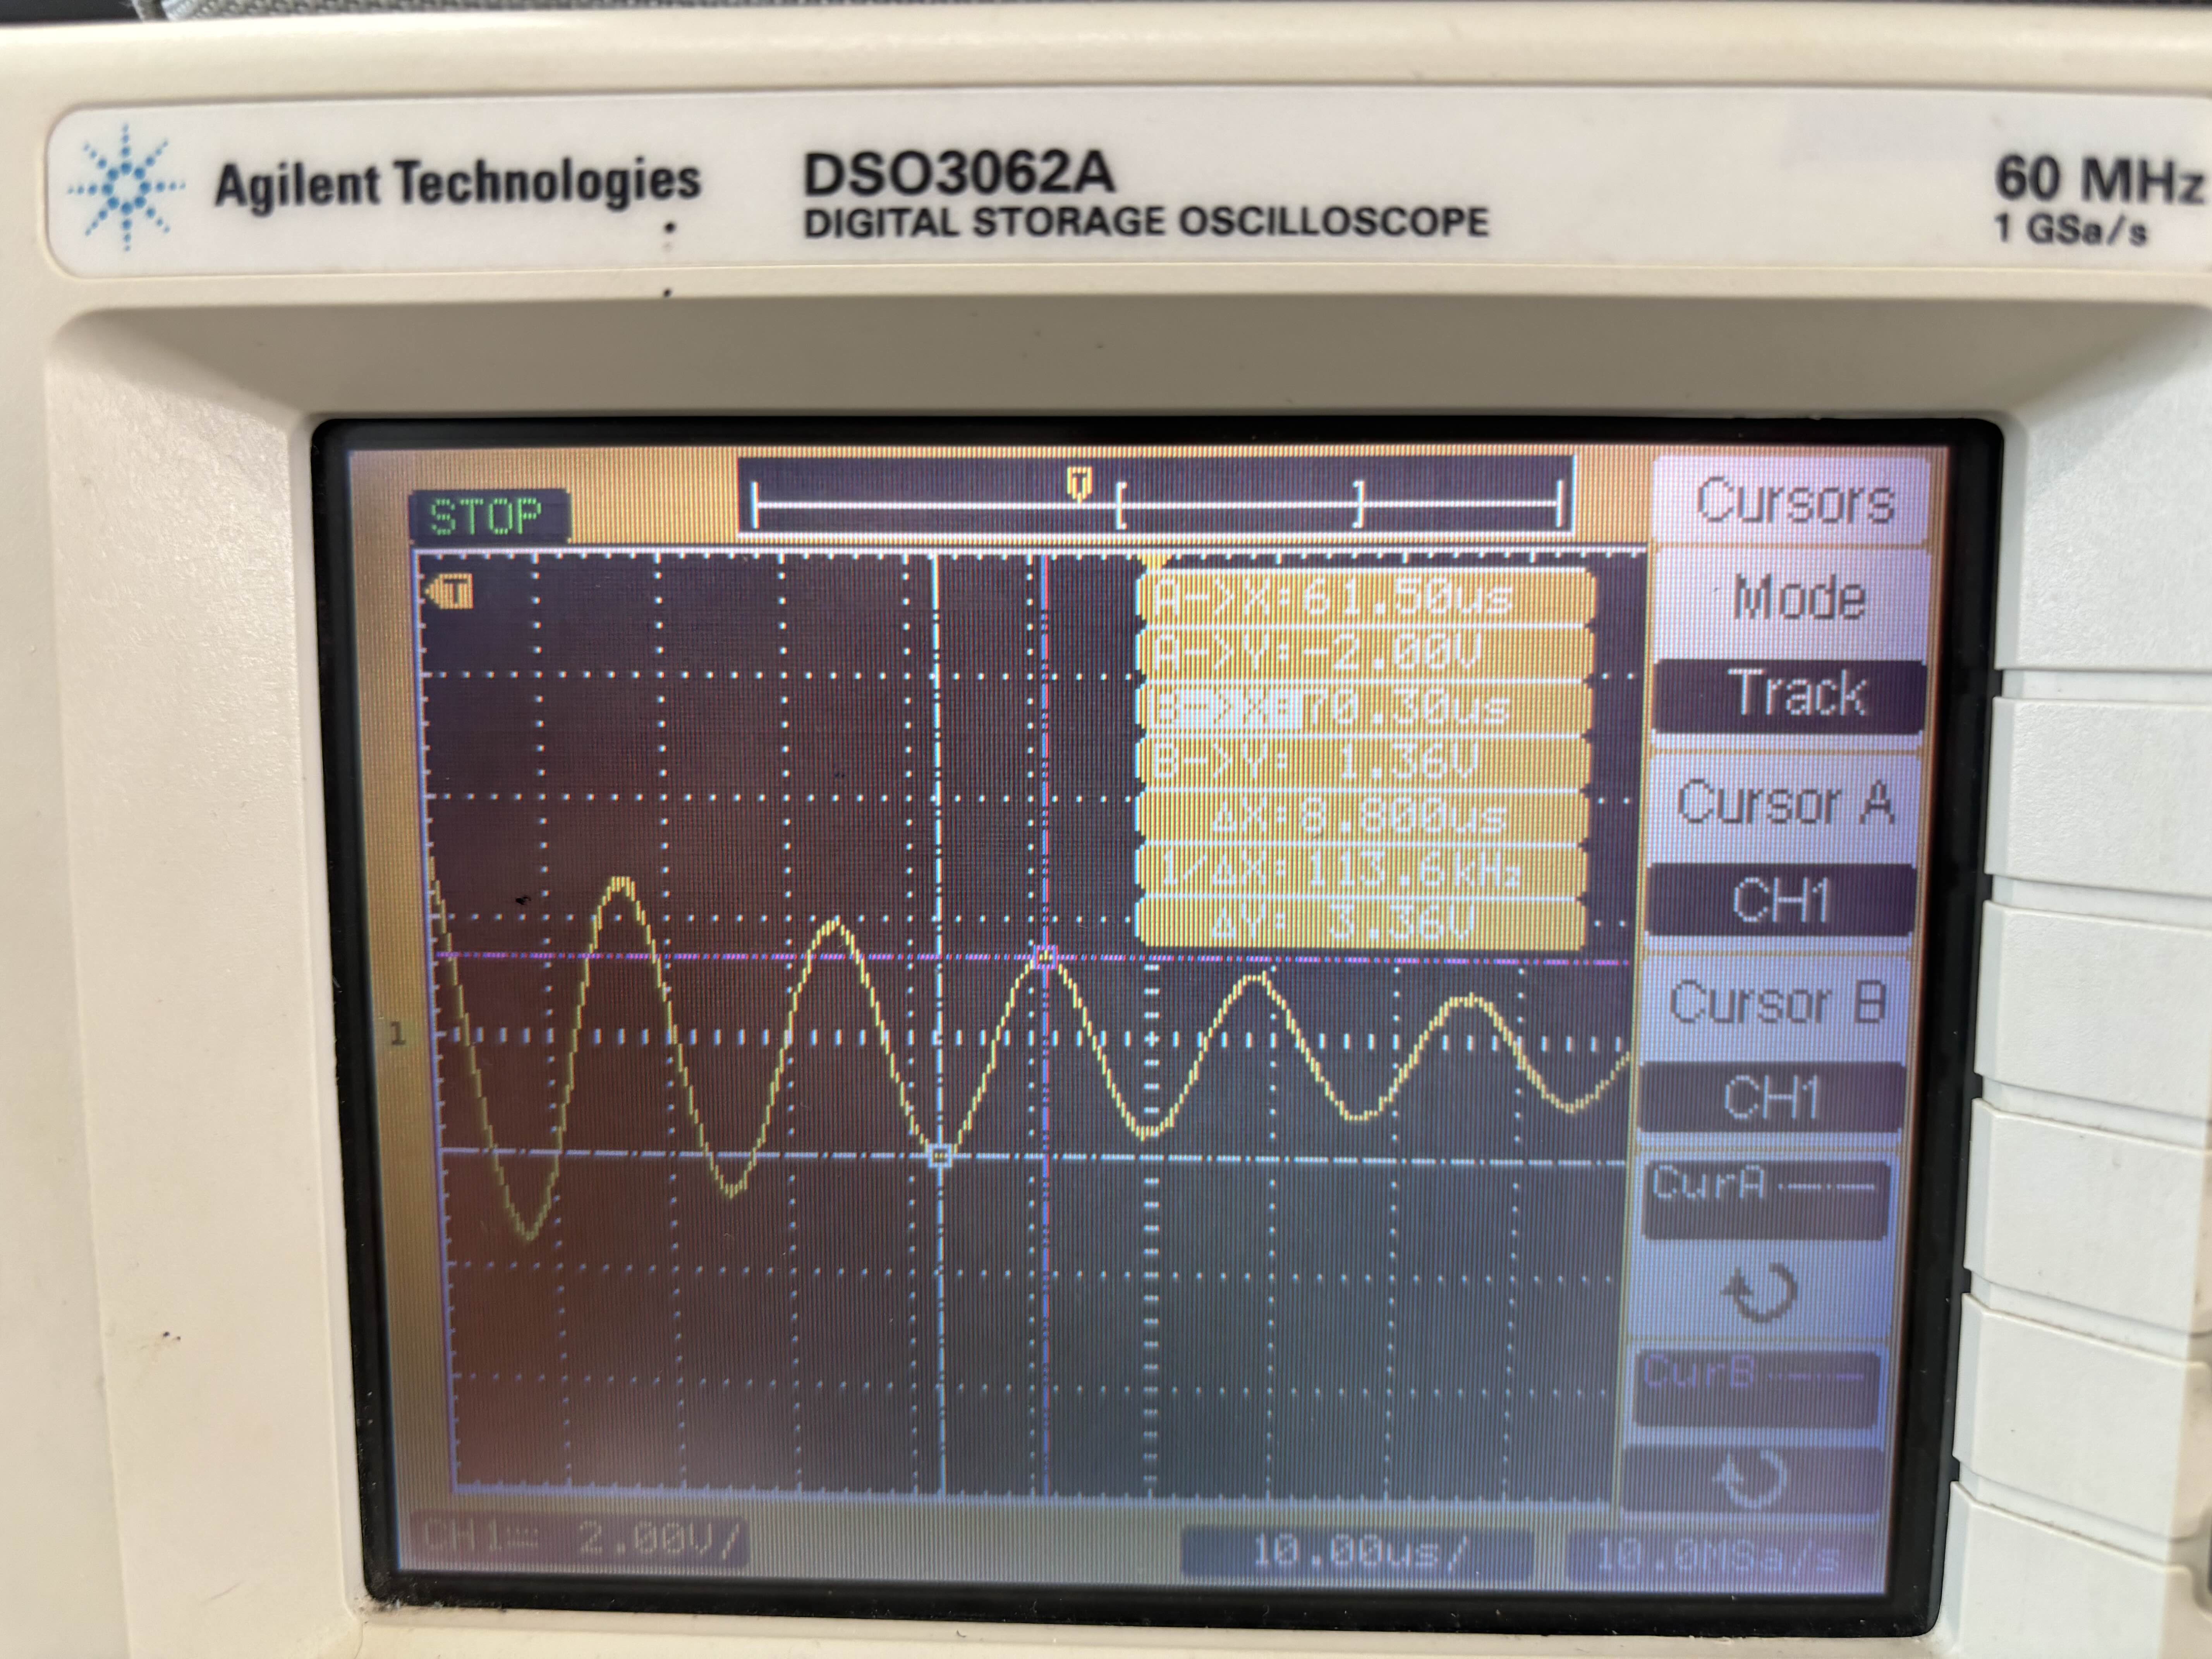
\includegraphics[width = 225pt]{figs/fig6.jpg}
	\end{subfigure}
\end{figure}
We know the value of $\omega_n, L, C$, we can use it to calculate $\xi$ from which we can calculate $R$ and verify. We can get $\xi$ from the equation, 
\begin{align*}
   V(t) &= \left(\frac{CV_{DC}}{\sqrt{1-\xi^2}} \right) e^{-\xi \omega_n t}\cos\left(\omega_d t + \tan^{-1}\left(-\frac{\xi \omega_n}{w_d}\right)\right). 
\end{align*}
On solving we get $R$ to be approximately equal to the theoretical value of $55\Omega$
\newline Python code used for verifcation can be found below,
\newline
\url{https://github.com/ArjunPavanje/EE1200/tree/main/Experiment_4/codes} 
\section{Conclusion}
In this experiment, we derived the equation for the damped oscillation of a series $LC$ circuit with internal resistance and verified it experimentally.
\end{document}
